\scanpage{231}
\mspage{181}
% L1–2
Écrivons la suite spectrale de Leray pour $f:X\to Y$ et $f^*F=F_X$ :
% L3
\[
H^{\unsure{n|m}}(X,f^*F)\Longleftarrow E^{pq}_2=H^p(Y,H^q(Z,\unsure{f^*F|F}))
\]
% L4–5
où ``$H^q(Z)$'' doit être vu comme un syst. local sur $Y$. Donc pour ($\alpha$) on a
% L6
\[
E^{pq}_2=0\quad\text{si }0<q<n
\]
% L5–6, right
\figure{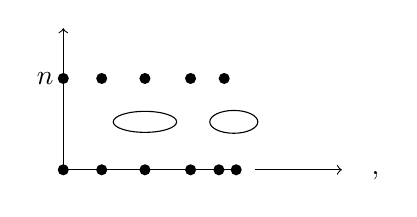
\begin{tikzpicture}[x=.61cm,y=.58cm]
\draw (0,0)--(3.6,0); \draw[->] (4.0,0)--(5.8,0);
\draw[->] (0,0)--(0,3.1);
\node[left] at (0,2.0) {$n$};
\foreach \x in {0,.8,1.7,2.65,3.24,3.6}{\fill (\x,0) circle (2pt);}
\foreach \x in {0,.8,1.7,2.65,3.35}{\fill (\x,2.0) circle (2pt);}
\draw (1.7,1.05) ellipse (.66 and .23); \draw (3.55,1.05) ellipse (.5 and .25);
\node at (6.5,-.12) {,};
\end{tikzpicture}}
% L7
donc on trouve la suite exacte
% L8–10
\[
\scriptstyle 0\to H^n(Y,F)\to H^n(X,\deleted{\unsure{f^*}}F_X)
\xrightarrow{\alpha}H^0(Y,\underbrace{H^n(Z,\overbrace{F_Z}^{\substack{M_Z\\\Vert}})}_{\substack{\Vert\\\mathrm{Hom}(\pi_n(Z,\unsure{z}),M)\\\text{par th. de Hurwicz}}})\longrightarrow H^{n+1}(Y,F)
\]
% L11–15
Ici \deleted{\unsure{$Z$}} je fixe un point $x$ de $X$, $Z$ désigne la fibre de $f$ en $y=f(x)$, et $M$ celle de $F$ en $y$, $M=F_y$. Le groupe $\pi_1(Y)$ y opère, d'ailleurs $\pi\overset{\mathrm{def}}{=}\pi_1(X,x)\unsure{\simeq|\xrightarrow{\sim}}\pi_1(Y,\unsure{y})$ aussi. Le $H^0(Y,H^n(Z,F_Z))$ peut s'interpréter, sauf erreur, comme
% L16
\[
\mathrm{Hom}_{\pi\deleted{\unsure{x}}}(\pi_n(Z;x),M),
\]
% L17–19
en tenant compte de l'opération de $\pi$ \inserted{$=\pi_1(X,x)$} sur $\pi_n(Z,\unsure{n|x})$ également. (À vérifier.) Il faut \unsure{interpréter} la flèche
% L20
\[
H^n(X,\deleted{\unsure{f^*}}F_X)\longrightarrow\mathrm{Hom}_{\pi}(\pi_n(Z,x),M),
\]
% L21
via l'application composée
% L22
\[
\pi_n(Z,z)\longrightarrow\pi_n(X,x)\longrightarrow H_n(X,\mathbb Z)
\tag*{(*)}
\]
% L23–24
Si $F$ est \uline{constant} sur $Y$ (p. ex. si $Y$ 1-connexe), donc de valeur $M$, on a les flèches can.
% L25–26
\[
\begin{aligned}
&\scriptstyle H^n(X,F_X)=H^n(X,M)\longrightarrow\mathrm{Hom}(H_n(X,\mathbb Z),M)\xrightarrow{\inserted{\text{grâce à la composition avec (*)}}}\mathrm{Hom}(\pi_n(Z,z),\\
&\hfill\scriptstyle M)
\end{aligned}
\tag*{($*'$)}
\]
% archive sheet number: 231
